\documentclass[a4paper, 14pt]{article}
\usepackage{comment}

\usepackage{setspace}
\usepackage{indentfirst}
%% Language and font encodings
\usepackage{extsizes}
\usepackage[english, russian, ukrainian]{babel}
\usepackage[utf8x]{inputenc}
\usepackage[T1]{fontenc}
\linespread{1.6}
%% Sets page size and margins
\usepackage[a4paper,top=2cm,bottom=2cm,left=3cm,right=2cm,marginparwidth=1.75cm]{geometry}

%\usepackage{fontspec}

%% Useful packages
\usepackage{authblk}
\usepackage{amsmath}
\usepackage{graphicx}
\usepackage[colorinlistoftodos]{todonotes}
\usepackage[colorlinks=true, allcolors=black]{hyperref}
\usepackage{tikz}
%\usepackage{subfigure}
\usepackage[lofdepth,lotdepth]{subfig}
\usepackage{float}
\usepackage{multirow}
\usepackage{hhline}
\usepackage{lineno}

%\linenumbers
\renewcommand{\thefigure}{\thesection.\arabic{figure}}

\numberwithin{equation}{section}
\numberwithin{table}{section}

\title{}


\author[1]{V. Haponov}
\author[2]{R. Yermolenko}
\affil[1]{Taras Shevchenko National University of Kiev, Kiev, Ukraine}
\affil[2]{}

\setcounter{Maxaffil}{0}
\renewcommand\Affilfont{\itshape\normalsize}
\renewcommand{\arraystretch}{1.5} %% increase table row spacing
%\renewcommand{\tabcolsep}{1cm}

\date{}
\begin{document}
\begin{titlepage}
\renewcommand{\baselinestretch}{1.0}
\selectlanguage{ukrainian}
\begin{center}
КИЇВСЬКИЙ НАЦІОНАЛЬНИЙ УНІВЕРСИТЕТ ІМЕНІ ТАРАСА ШЕВЧЕНКА\\Фізичний факультет\\Кафедра ядерної фізики
\end{center}
\vspace*{1.5cm}
{}\hfill\mbox{На правах рукопису}

\vspace*{3cm}
\begin{center} {\bf
}
\end{center}
\medskip
\vspace*{0.7cm}
	\begin{flushleft}
		\parbox{12cm}{
		\textbf{Галузь знань:} 10 <<Природничі науки>>
		
		\textbf{Освітня програма} - Фізика
		
		\textbf{Спеціальність} - 104 <<Фізика та астрономія>>
		
		\textbf{Спеціалізація} Ядерна енергетика
		}
	\end{flushleft}
\renewcommand{\baselinestretch}{1.5}
\vspace*{1cm}
{}\hfill\hspace{7.5cm}\parbox{9cm}{\textbf{Кваліфікаційна робота бакалавра}\\
студента 4 курсу\\ Гапонова Валентина Вікторовича \\ \\ 
\textbf{Науковий керівник} \\ доц. ф.-м. наук\\ Єрмоленко Руслан Вікторович}
\bigskip


\vfill
{\small \noindent
Робота заслухана на засіданні кафедри ядерної фізики та рекомендована до захисту на ЕК, протокол , протокол № \underline{\hspace{1.0cm}}  від <<\underline{\hspace{1.0cm}}>> \underline{\hspace{3.5cm}}2020 р.\\[0.4cm]
Завідувач кафедри \hspace{9 cm} Каденко І. М.}
%\bigskip
\vfill
\begin{center} Київ, 2020 \end{center}

\end{titlepage}

\begin{titlepage}
\renewcommand{\baselinestretch}{1.0}
\selectlanguage{ukrainian}
\newcommand{\ul}[1]{\rule{#1}{0.1pt}}
	\begin{spacing}{1.8}
		\vspace*{4.5cm}
		{\center
		{\bf ВИТЯГ}\\
		з протоколу № \ul{2.4cm}\\
		засідання Екзаменаційної комісії\\[2cm]}
		{\noindent
		Визнати, що студент \ul{7.2cm} виконав та захистив кваліфікаційну роботу бакалавра з оцінкою \ul{7.2cm} .\\[1cm]}
		{\flushright
		Голова ЕК \ul{7.8cm}\\
		<<\ul{1cm}>> \ul{4cm} 2020 р.\\}
	\end{spacing}
\end{titlepage}

%{\renewcommand{\baselinestretch}{1.2}

\pagestyle{empty}

\section*{Анотація}

{\bf Гапонов В.В.} ""\\
{\itshape Кваліфікаційна робота бакалавра за напрямом підготовки 6.040203 --- Фізика, спеціалізація «Ядерна енергетика». --- Київський національний університет імені Тараса Шевченка, фізичний факультет, кафедра ядерної фізики. --- Київ, 2020.} \\
{\itshape \bfseries Науковий керівник:} д. ф.-м. н. Єрмоленко Р.В.%[0.5cm]
\\[0.5cm]
\\
{\bf Ключові слова:} Нейтронно активаційний аналіз, германиєвий детектор, метод Монте Карло\\   

\newpage
\thispagestyle{empty}
\selectlanguage{english}
\section*{Summary}

{\bf Haponov V.V.} ""\\
{\itshape Qualifying work of the bachelor on a speciality 6.040203 --- physics, specialization "Nuclear power". --- Taras Shevchenko National University of Kyiv, Faculty of Physics, Department of Nuclear Physics. --- Kyiv, 2020.\\}
{\itshape \bfseries Research supervisor:} Dr. R. Yermolenko.
\\[0.5cm]
{\bf Key words:}.

%content
\selectlanguage{ukrainian}
\newpage
\tableofcontents
\newpage
\pagestyle{plain}
\setcounter{page}{2}
	
%end 
\newpage
\section{Вступ}

З розвитком технологій та промисловості, забрудненням навколишнього середовища, ростом популяції населення, все частіше починає підніматись питання нестаці вичерпання природних ресурсів. Особливо гостро це торкається невідновлюваних природніх ресурсів. З кожним роком вичерпаних родовищ стає все більше. Так, наприклад, по оцінкам "Римського клубу": запасів алюмінієвих руд вистачить на 55 років, міді - 49 років, заліза - 173 роки, свинцю - 64 роки, хрому - 154 роки Це змушує шукати нові родовища.

З іншого боку 3/4 поверхні планети вкриті океанми, а по різним данним дослідженно від 5\% до 7\% дна.
Океанічне ложе має плоский або горбистий рельєф, та в основному від 3,5 - 6 кілометрів глибини, але зустрічаються глибоководні жолоби до 11 кілометрів в глибину, їх найбільше Тихому океані. 

Зарахунок досить складних умов і високого тиску, стандартні методи аналізу мінеральних порід за допомогою габаритного обладнення є дуже складними, а в деяких місцях такий єтап пошуку родовищ як буріння опорних та параметричних свердловин є не можливим.

На основі проекту SABAT(Stoichiometry Analysis By Activation Techniques) - за мету в якому було поставлено пошук небезних речовин на дні Балтійского моря з використання нейтронно активаційного аналізу для неінвазивного дослідження обьекту. Я допустив можливість використання данного методу дослідження для отримання більш розгорнутої інформації про океанічне дно.	


\setcounter{figure}{0} 
\newpage
\section{Розділ 1}
\setcounter{figure}{0} 
\subsection{Мультипоточність Geant4}
Geant4 - написаний на об'єктно орієнтованій мові програмування С++, яка дає можливість використовувати мульти-поточну архітектуру, і отримувати більшу продуктівність коду. При переносі процесу в інший потік, під процес бути виділене ядро тільки в тому випадку якщо воно не зайнете іншим процесом, це призводить до зменшення швидкості виконня при збільшенні кількості потоків. 

При використанні мульти-поточної архіектури обов'язково необхідно дбати про синхронізацію потоків для безпечного виконання коду. Geant4 - використовує G4MTRunManager - данний клас наслідується від базового G4RunManager - але включає в себе реалізацію пулу потоків, це дає змогу контролювати кожен з об'єктів які створюється в рамках пулу, та валідувати їх. 

Так як при моделюванні потрібно щоб кожен запуск відбувався з однаковими параметрами та за тієї ж самої геометрії, необхідно щоб класи інтерфейсу які відповідають за створення данних об'єктів були доступні для всіх об'єктів пулу.

\subsection{$QGSP\_BERT$}
	$QGSP\_BERT$ - ця фізична модель входить в перелік стандартних фізичних моделей розрахункового пакету Geant4
	Базується на каскадній моделі Бертіні та враховує реакції для нейтронів менше ніж 20 МеВ. Для валідації данної моделі необхідне виконання наступних умов $\frac{\lambda_B}{\nu} \ll \tau_c \ll \Delta{t}$, $\lambda_B$ - хвиля де-Бролля для налітаючої частинки, $\nu$ - швидкість налітаючої частинки, $\Delta{t}$ - час між зіткненнями. Та модель яка лягла в основу коду Geant4 була протестована на частинках з енергіями від 100 МеВ до 3 ГеВ
\subsection{Джерела нейтронів}
	Джерела 

\newpage
\section{Розділ 2}
\setcounter{figure}{0}
В рамках данного моделювання були розглянуті матеріали розглянуті в Таб.~\ref{tabl:Materials}.
\begin{table}[h]
	\centering
	\begin{tabular}{|c|c|c|}
		\hline
		Назва & Хімічна склад & Ізотопний склад \\
		\hline
		Гірчичний газ & $C_4H_8Cl_2S$ & $C^{12}$, 	$H^1$, $Cl^{35}$, $S^{22}$ \\
		\hline
		Ютенбогардтит & $Ag_3AuS_2$ & $Ag^{108}$ , $Au^{197}$ , $S^{32}$ \\
		\hline
		Халькопірит & $CuFeS_2$ & $Cu^{64}$, $Fe^{56}$, $S^{22}$ \\
		\hline
		Збіднений уран & U & 99.27\% $U^{238}$, 0.7\%$U^{235}$, 0.005\%$U^{234}$\\
		\hline
	\end{tabular}
\caption{Елементи та ізотопи які вхьодять до їх складу} 
\label{tabl:Materials}
\end{table}

Найбільш інтенсивні піки для кожного з елементів розглянуті в Табл. ~\ref{tabl:ElementsEnergy}, використовувались елементи з бази доступної в Geant4
\begin{table}[h]
\centering
	\begin{tabular}{|c|c|} 
		\hline
		Елемент& Енергія, МеВ \\
		\hline
		$Cl$ & 0.79, 1.17, 1.94, 2.12, 6.12, 7.79, 8.58 \\
		\hline
		$H$ & 2.23 \\
		\hline
		$C$ & 4.44 \\
		\hline
		$Fe$ & 7.64, 9.30 \\		
		\hline
		$S$ & \\
		\hline
		$Cu$ &  \\
		\hline
		$U$ & 1.26\\
		\hline
		$Ag$ &  0.8, 2.89, \\
		\hline
		$Au$ & 0.67, 1.087, 2.24, 1.37  \\
		
		\hline
	\end{tabular}
\caption{Таблиця енергій найбільш інтенсивних піків} 
\label{tabl:ElementsEnergy}
\end{table}

\subsection {Геометрії моделювання}
Змодельована геометрія схожа на ту яка використовувалась у проекті SABAT Рис. ~\ref{ris:SabatG}, але с наступними відмінностями: по-перше не моделювався корпус самої сабмарини так як в він не ніс жодного корисного навантаження припроведені розрахункі, детектор та джерело були рознесені на дещо більшу відстань, та поміняні місцями, також на данному єтапі було вирішено відмовитись від моделювання морського дна, так як це дуже суттева знижувало ефективність виконання коду. Також було приділено більшу увагу моделюванню захисту детектора.
\begin{figure}[hbt!]
	%\vspace{-10pt}
	\centering 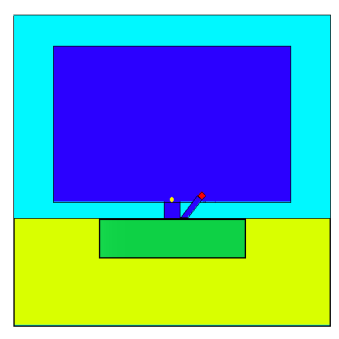
\includegraphics[width=0.7\textwidth]{images/sabatGeometry.png}
	\caption{Геометрія проекту SABAT} 
	\label{ris:SabatG}	
\end{figure}

Геометрія яка використовувалась для набору спектрів зоображена на Рис. ~\ref{ris:Geometry}, довжина ребра кубу середовища 1 м., довжина ребра бічної поверхні мішені(коричневий паралелепіпед) 40 см., від мішені до чутливого об'єму детектора 30 см., від чуливого об'єму до джерела 30 см., матеріал середовища був взятий с запропонованою бази матеріалів Geant4 - "G4\_WATER". Джерело нейтронів поміщене в напрявляючий об'єм(червоний циліндр), який виготовлений з токого шару свинцю. Чутливий об'єм детектора поміщений у захист зі свинцю, бору, та алюмінія, направляючі об'єми заповнені повітрям(G4\_AIR)
\begin{figure}[hbt!]
	%\vspace{-10pt}
	\centering 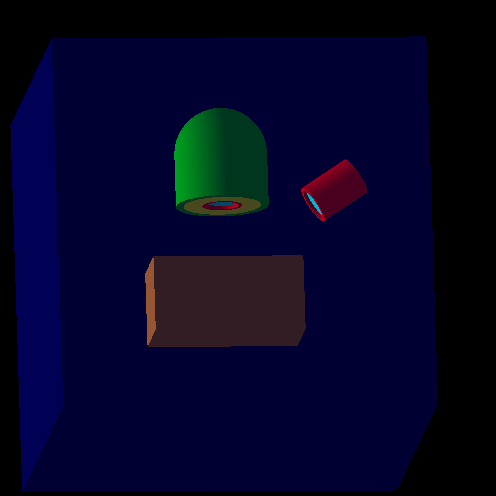
\includegraphics[width=0.7\textwidth]{images/geometryAll.png}
	\caption{Геометрія моделі} 
	\label{ris:Geometry}	
\end{figure}

Для спрощення моделювання точкове джерело нейтронів було розміщенне всередині набравляючого кооксіального об'єму Рис. ~\ref{ris:Geometry} (червоного кольору), під кутом для того щоб більша кількість нейтронів потрапляла в поверхню яка безпосередню знаходиться під чутливим об'ємом детектора 


\subsection{Чутливий об'єм детектора та захист}
	
	Для моделювання чутливого об'єму був обраний надчистий германій, з діаметром 60.6 міліметрів, та довжиною 56.7 міліметрів. Рис. ~\ref{ris:s_detector_volume} 	
	\begin{figure}[hbt!]
		%\vspace{-10pt}
		\centering 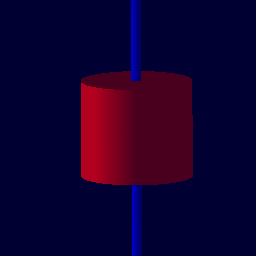
\includegraphics[width=0.7\textwidth]{images/sDetector158cm3.png}
		\caption{Форма чутливого об'єму} 
		\label{ris:s_detector_volume}	
	\end{figure}

	Детектор буде розміщенний поряд з джерелом нейтронів високих енергій, 14.5 МеВ. Тому детектор був розміщений у трьох шаровий захист. Рис. ~\ref{ris:s_detector_P}	
	\begin{figure}[hbt!]
		%\vspace{-10pt}
		\centering 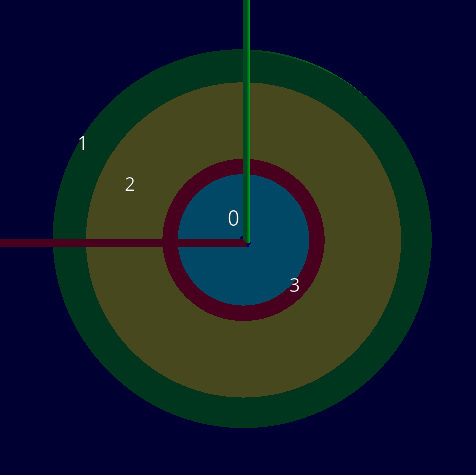
\includegraphics[width=0.7\textwidth]{images/dectorPrt.png}
		\caption{Захист детектора, Al - зелений товщина 2 см., B - жовтий товщина 5 см., Pb - червоний товщина 1 см. Блакитний шар повітря} 
		\label{ris:s_detector_P}	
	\end{figure} 

	В захисті використовується Бор для поглинання теплових нейтронів, так як вся детекторна система буде знаходитися під водою, то нейтрони від джерела будуть втрачати енергію при пружному розсіянні на водню. 
	
	Для поглинання теплових нейтронів перед чутливім об'ємом детектора був обраний $B^{10}$. Використовується в ТВЕЛ-ах для контролю кількості теплових нейтронів в активній зоні реакторної установки ВВЕР. 
	$B^{10} ( n, \alpha \gamma)Li_3^7$, Переріз захоплення нейтрона $B^{10} \ \sigma = 3380$ барн.
	$E_\gamma$ = 480 кеВ, реація з вильотом $\gamma$ - кванту протікає з ймовірністю 94\%.
	
	Для зовнішнього корпусу захисту чутливого об'єму використовувався $Al^{26}$ - товщиною 1 см на Рис. ~\ref{ris:s_detector_P} - зоображений зеленим кольором 
	
	За приклад було взято детектор N21879A виробника від ORTEC AMETEK, параметри розмірів були взяті від офіційного дестрибютера.
	
\subsection{Опис коду моделі}
Цілью було написати максимально зручний код для набору спектрів за різних умов та на різних мішеннях, тому були створені абстрактні класси для створення геометричних об'єктів. Для зручності створення матеріалів були створенні структури. 
Та для пришвидшення роботи були всі можливі константи ініціалізувалися на етапі компіляції. Для полегшення контролю над пам'яттю використовувалися розумні вказівники С++ 14 стандарту. Архітектура коду моделювання зоображена на Рис. ~\ref{ris:s_classDiagram} 
\begin{figure}[hbt!]
	%\vspace{-10pt}
	\centering 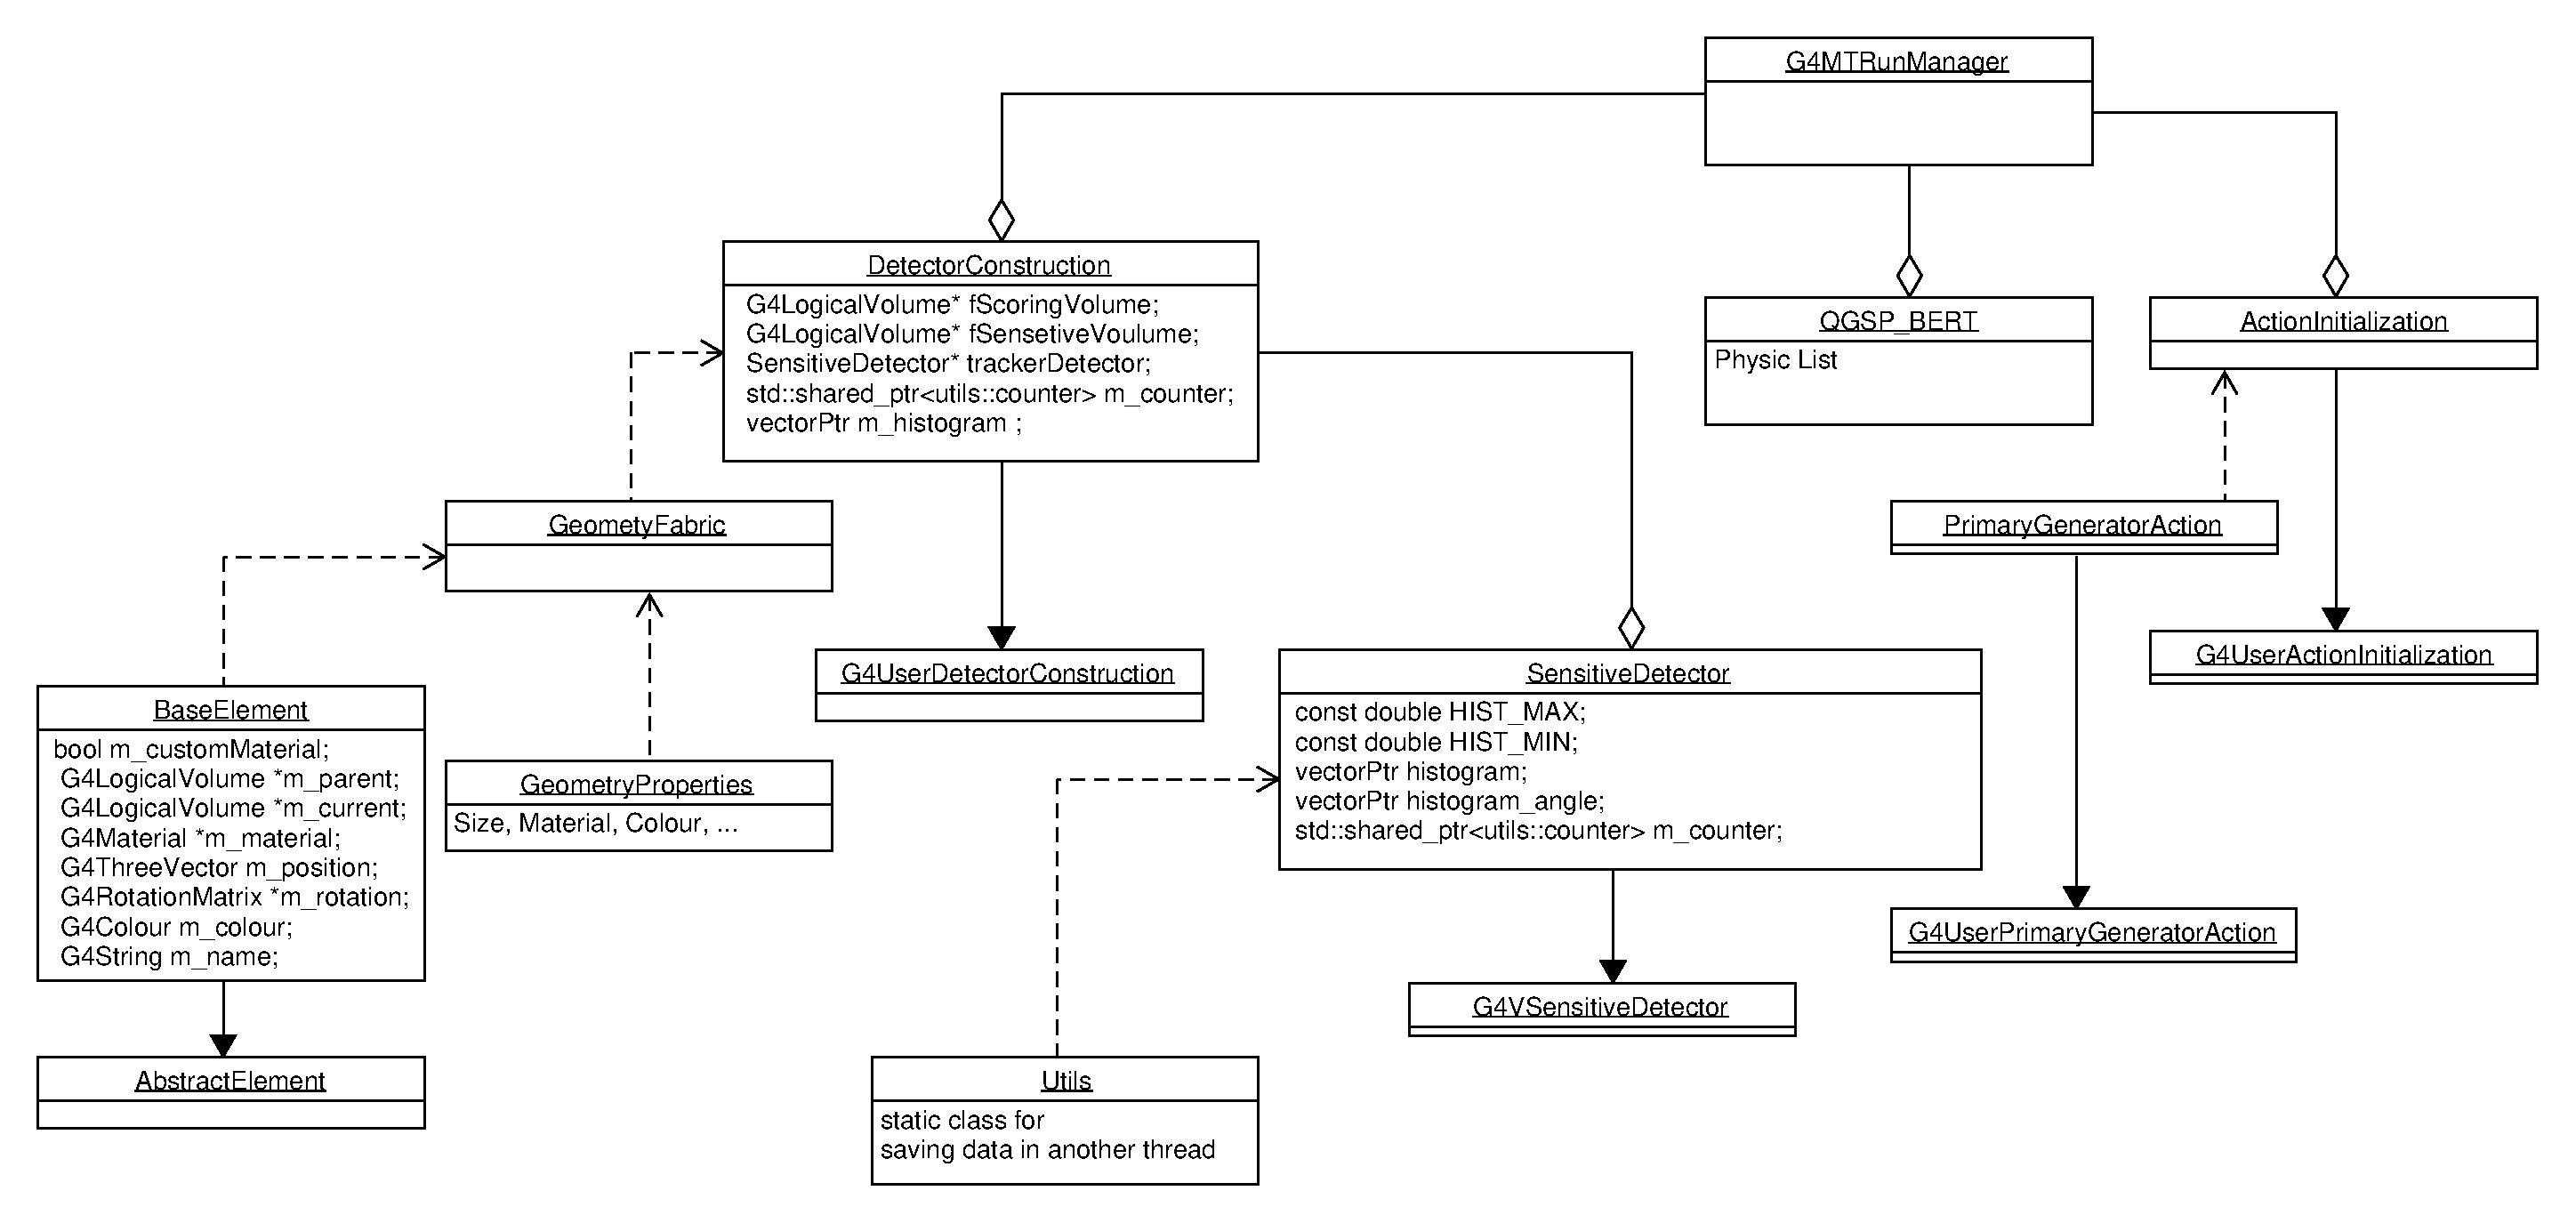
\includegraphics[width=1\textwidth]{res/classDiagram.pdf}
	\caption{Діаграма класів коду моделі} 
	\label{ris:s_classDiagram}	
\end{figure} 

	
\newpage 
\section{Розділ 3}
\setcounter{figure}{0}
\subsection{Опис обробки спектру}

В результаті моделювання, чутливим об'ємом набирались апаратні спектри, для чутливого об'єму було встановленно 16384 біни. Далі для наближення спектру до реального, була проведенне його сглажування за наступної формулою $\Delta{E} = 2.36 \sqrt{F  \frac{w}{E}}  w$, $\Delta{E}$ - енергія на один бін, F - Фано фактор, w - кількість енргії на утворення пари, та пронормований на кількість нейтронів з джерела. Так як для спрощення побудови джерела в моделі, використовувалась спрощенна геометрія, а генерація нейтронів відбувалась майже строго у заданому напрямку. Так як джерело нейтронів вважалося ізотропним, то загальна кількіть частинок розраховувалась наступною формолую $ 4 \pi n = N$, де $N -$ це загальна кількість чатсинок.

Фон Рис. ~\ref{ris:FonPicks} набирався за тих тої самої геометрії Рис. ~\ref{ris:SabatG}, але за відсутності мішені(коричневий паралелепіпед), У фоні були проаналізовані наступні три піки: H з $E_\gamma = 2.23 MeV$, та два піки які отримались за рахунок захоплення нейтронів $Ge$ з $E_\gamma = 0.56MeV$, $E_\gamma = 1.44 MeV$ - це означає що данної геометрії частина нейтронів від джерела проходячи через захист потрапляє в чутливий об'єм детектора, та призводить до його руйнації. 
\begin{figure}[hbt!]
	%\vspace{-10pt}
	\centering 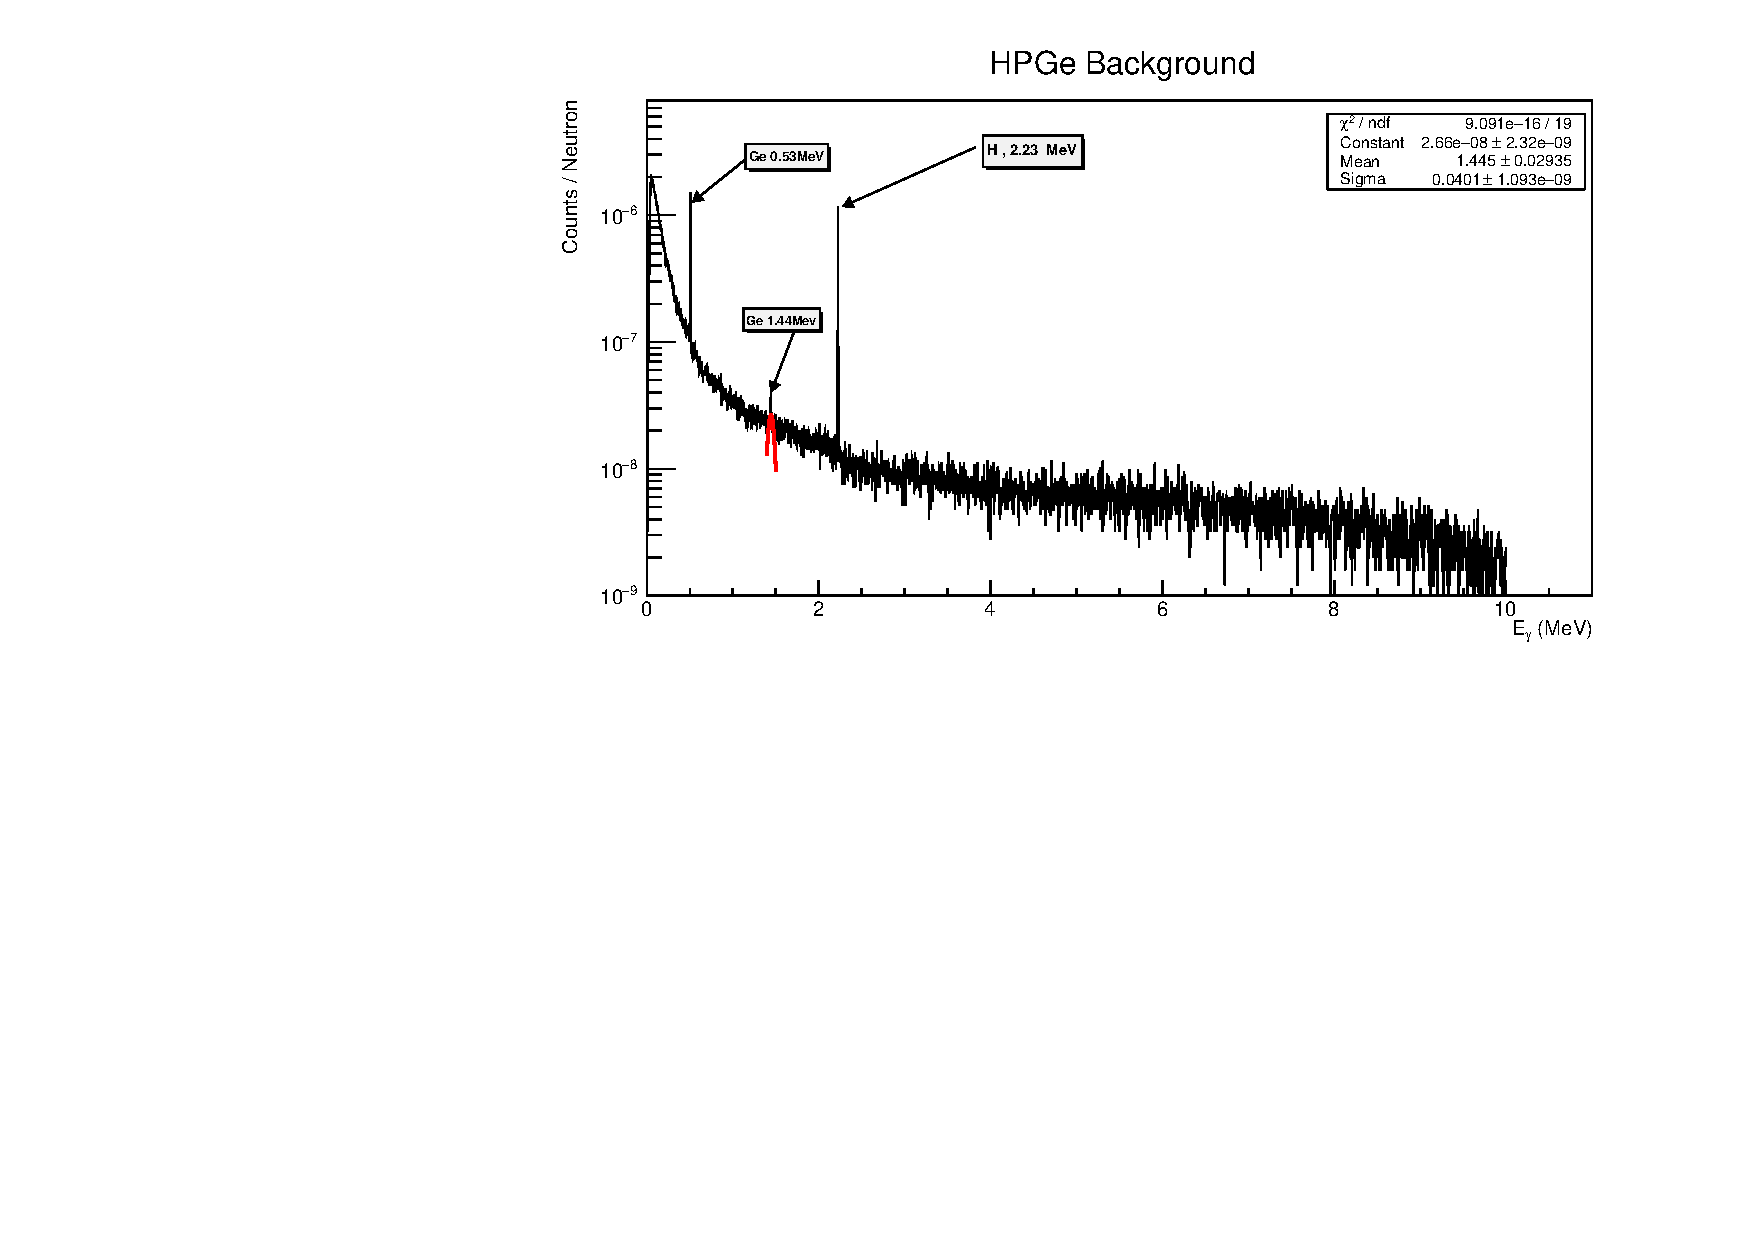
\includegraphics[width=1\textwidth]{res/smFonPiscks.pdf}
	\caption{Фон} 
	\label{ris:FonPicks}	
\end{figure} 


\subsection{Валідація моделі}

	Для підтвердження можливості проведення наборів на моїй моделі був набраний спектор для Гірчичного газу. Рис ~\ref{ris:MustBackAllLogSm}. Та порівняний з отриманим спектром в статьї <link to source ?help> 	
	\begin{figure}[hbt!]
		%\vspace{-10pt}
		\centering 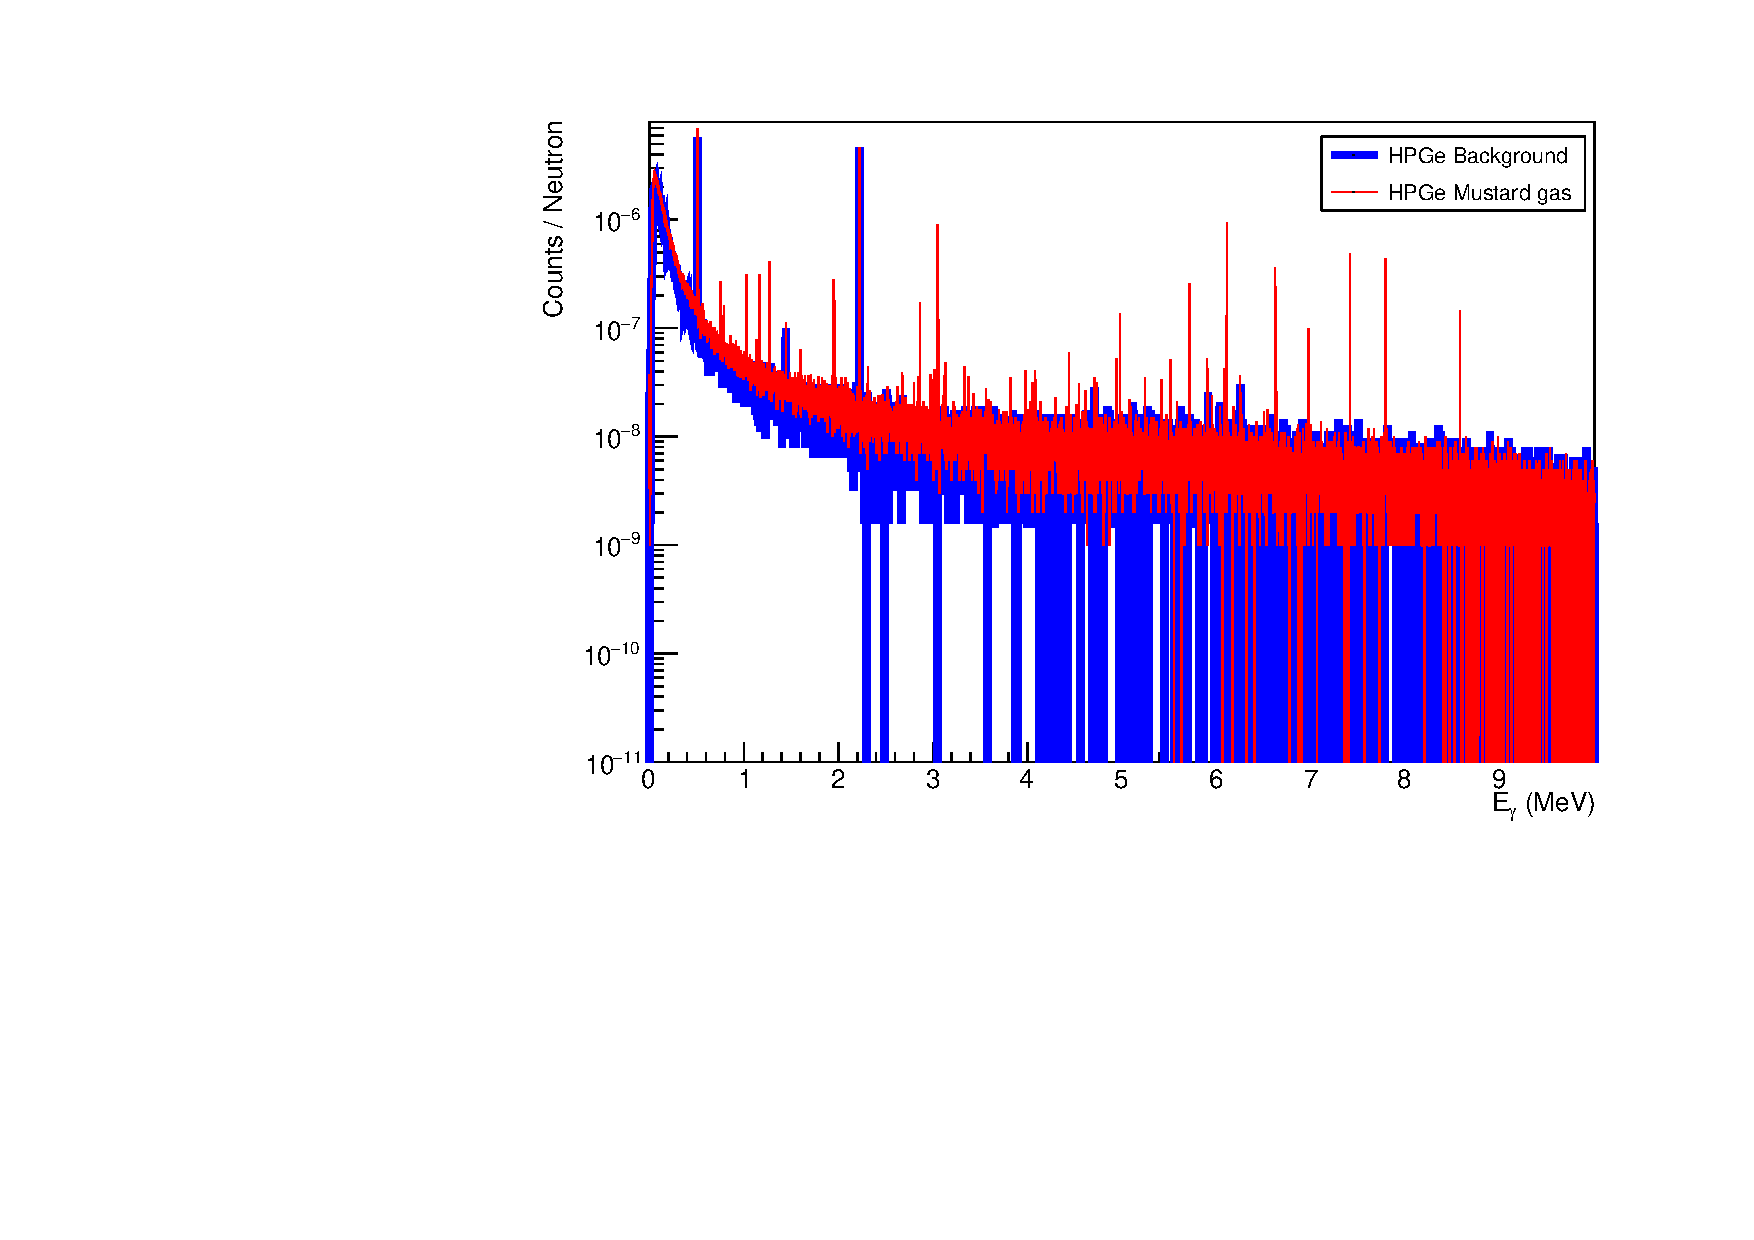
\includegraphics[width=1\textwidth]{res/smMustFonAll.pdf}
		\caption{Червоним - представлений спектор для Гірчичного газу. Синім - фону} 
		\label{ris:MustBackAllLogSm}	
	\end{figure} 
	У висновках до проведеної роботи в данної статьї було вказано, що най більш вираженими і читкіми були лінії Cl 7,42 7,80 8,58 МеВ, також було вказано ряд ліній які їм не вдалося валідувати (перефразувати "лінії") 
	На Рис. ~\ref{ris:MustFon78} - зоображені піки 7.42 та 7.80 МеВ
	Рис.  ~\ref{ris:MustFon89} - 8.58 МеВ	
	\begin{figure}[hbt!]
		%\vspace{-10pt}
		\centering 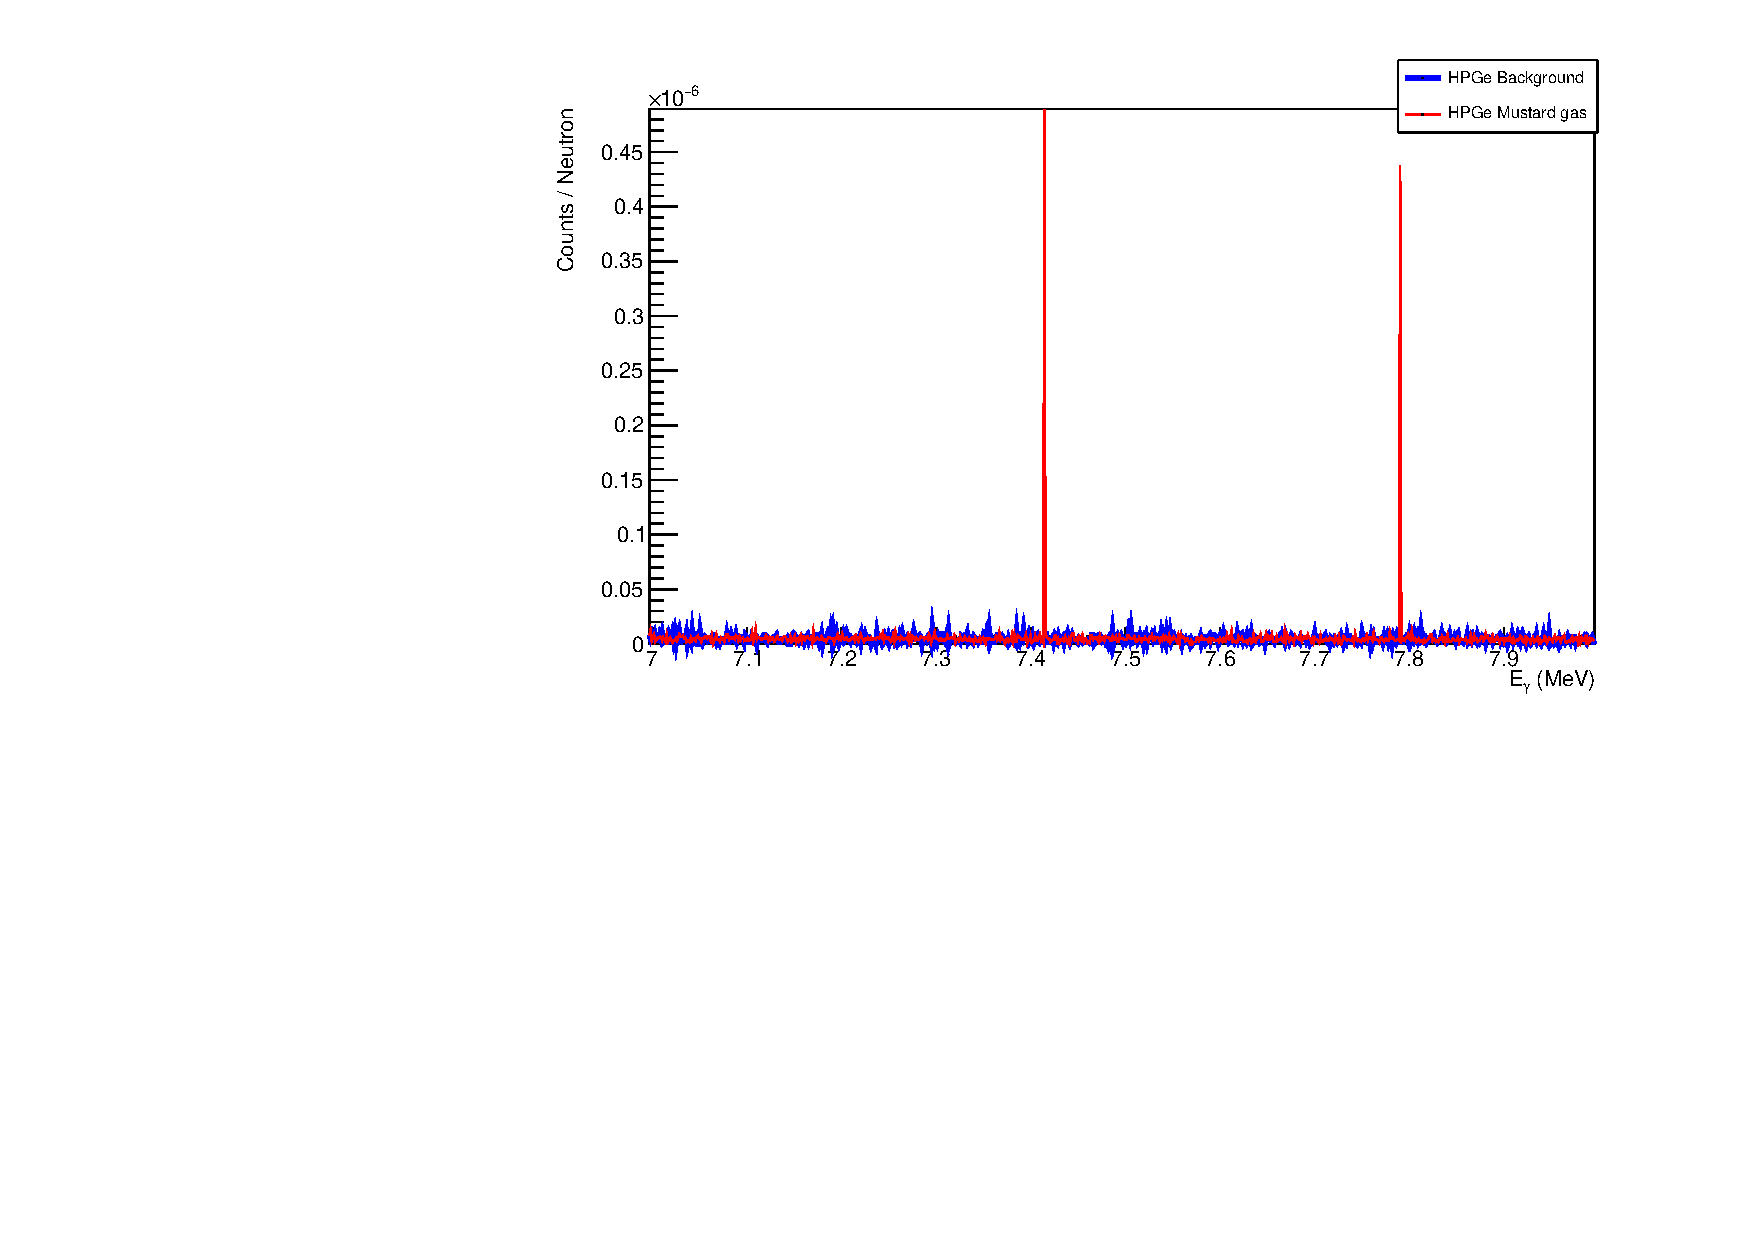
\includegraphics[width=1\textwidth]{res/mustFon78.pdf}
		\caption{Червоним - представлений спектор для Гірчичного газу. Синім - фону} 
		\label{ris:MustFon78}	
	\end{figure} 	
	\begin{figure}[hbt!]
		%\vspace{-10pt}
		\centering 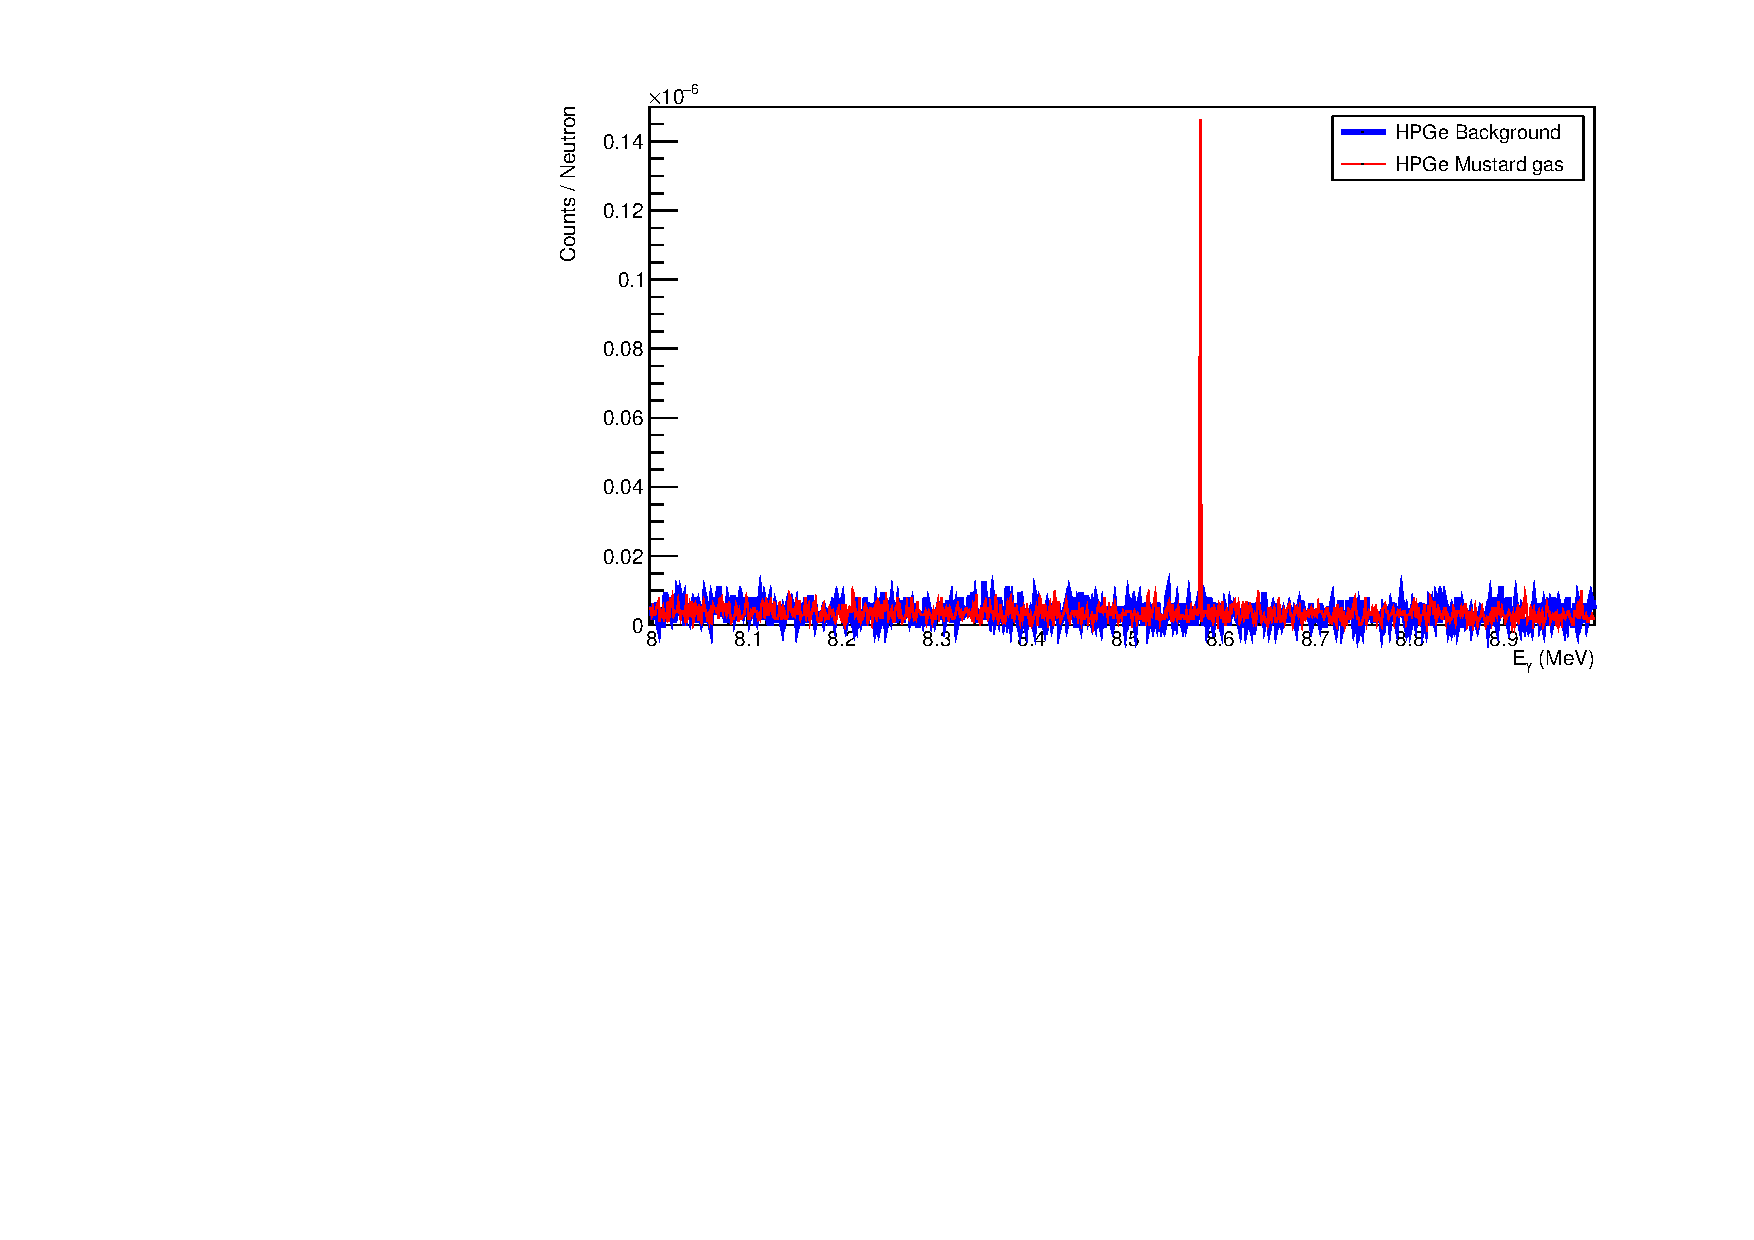
\includegraphics[width=1\textwidth]{res/mustFon89.pdf}
		\caption{Червоним - представлений спектор для Гірчичного газу. Синім - фону} 
		\label{ris:MustFon89}	
	\end{figure} 
	
\newpage

\subsection{Аналіз спектрів $Ag_3AuS_2$}

	За матеріал було обрано ютенбогардтит $Ag_3AuS_2$ - родовища з данними мінералами були знайдені на камчатці поблизу побережжня. Данний мінерал відноситься до рідкисних золотоносних руд, зустрічаеться в природі у твердому стані. Був знайдений на Камчатських родовищах. Рис. ~\ref{ris:Ag3AuS2Fon}	
	\begin{figure}[hbt!]
		%\vspace{-10pt}
		\centering 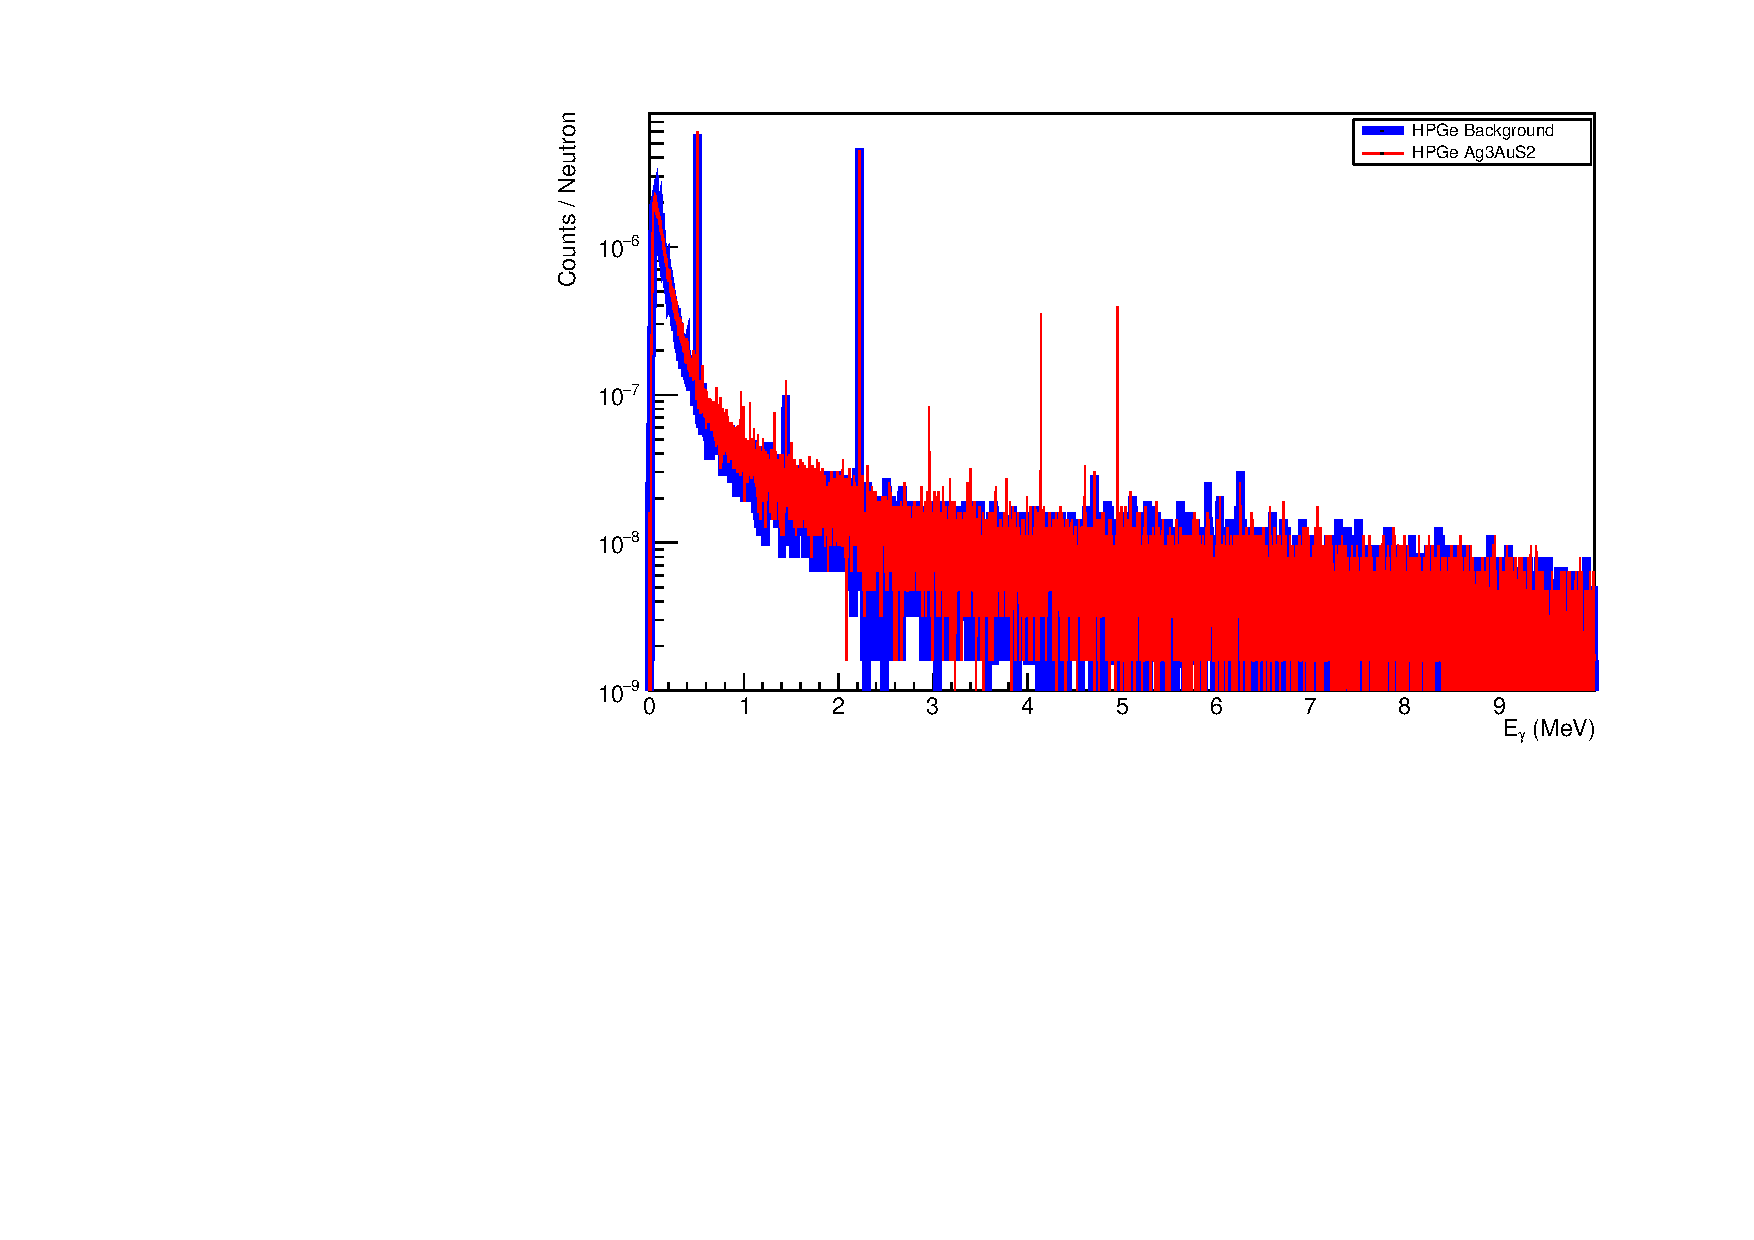
\includegraphics[width=1\textwidth]{res/auFonAllLog.pdf}
		\caption{Червоним - представлений спектор для $Ag_3AuS_2$. Синім - фону} 
		\label{ris:Ag3AuS2Fon}	
	\end{figure} 	
	Данний спектор і фон були набрані при опроміненні нейтронами з джерела максимальної енергією 14.5 МеВ
	Для порівняння було проведенно опромінення за допомгою нейтронів енергією 8.5 та 2.8 МеВ. Рис. ~\ref{ris:Ag3AuS28_5MeV}
	\begin{figure}[hbt!]
		%\vspace{-10pt}
		\centering 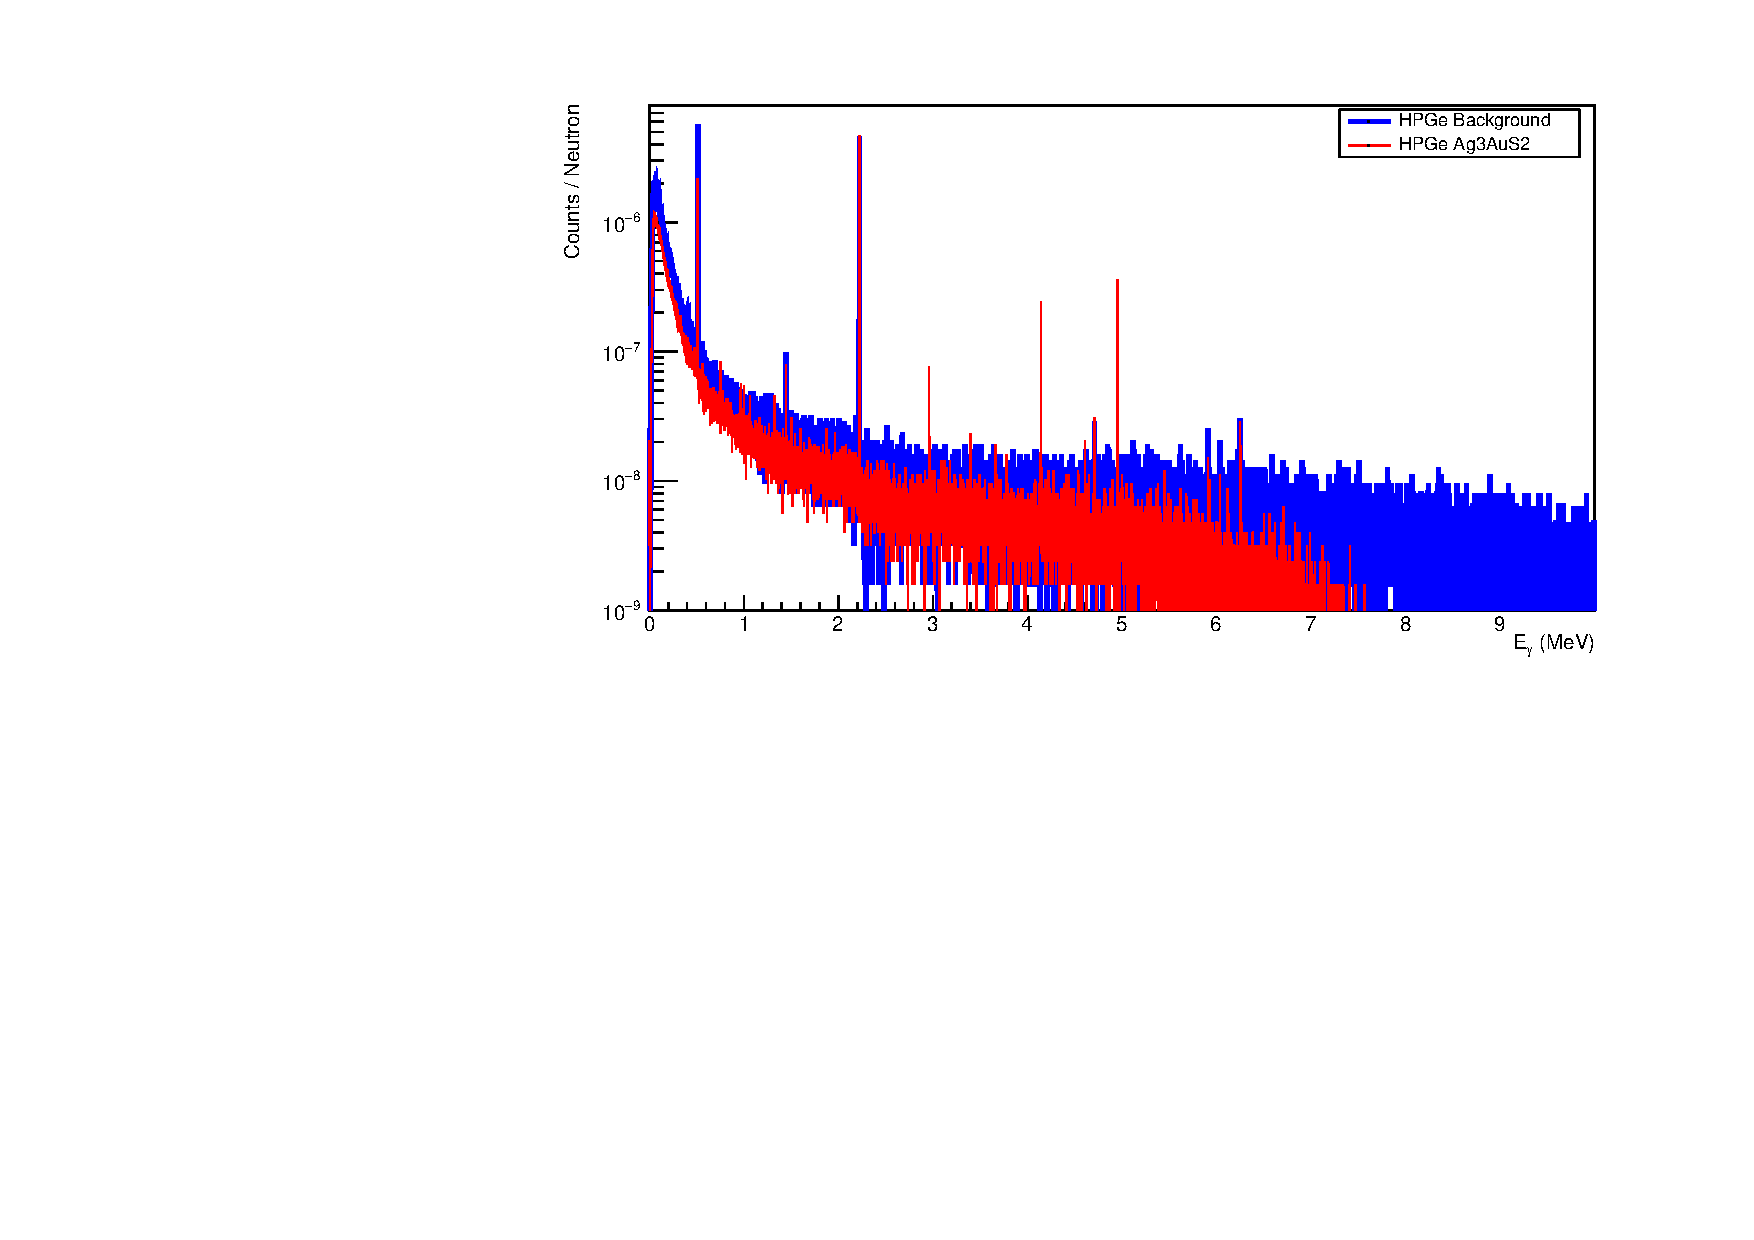
\includegraphics[width=1\textwidth]{res/Ag3AuS2_8_5MeVFonClasic.pdf}
		\caption{Червона - лінія спектру, набраного за опромінення нейтронами 8.5 МеВ}
		\label{ris:Ag3AuS28_5MeV}	
	\end{figure} 	
	Піки по близу 3, 4 і 5 МеВ майже не втратили інтенсивності тому саме вони були взяті в подальшу обробку. На данному графіку був взятий фон з опромінення 14.5 МеВ нейтронами. Рис. ~\ref{ris:Ag3AuS28_5MeV}
	Для того щоб проаналізувати залежність можливості використання ізотопних джерел був набраний спектор, за енергій нейтронів 2.8 МеВ Рис. ~\ref{ris:Ag3AuS22_8MeV}
	\begin{figure}[hbt!]
		%\vspace{-10pt}
		\centering 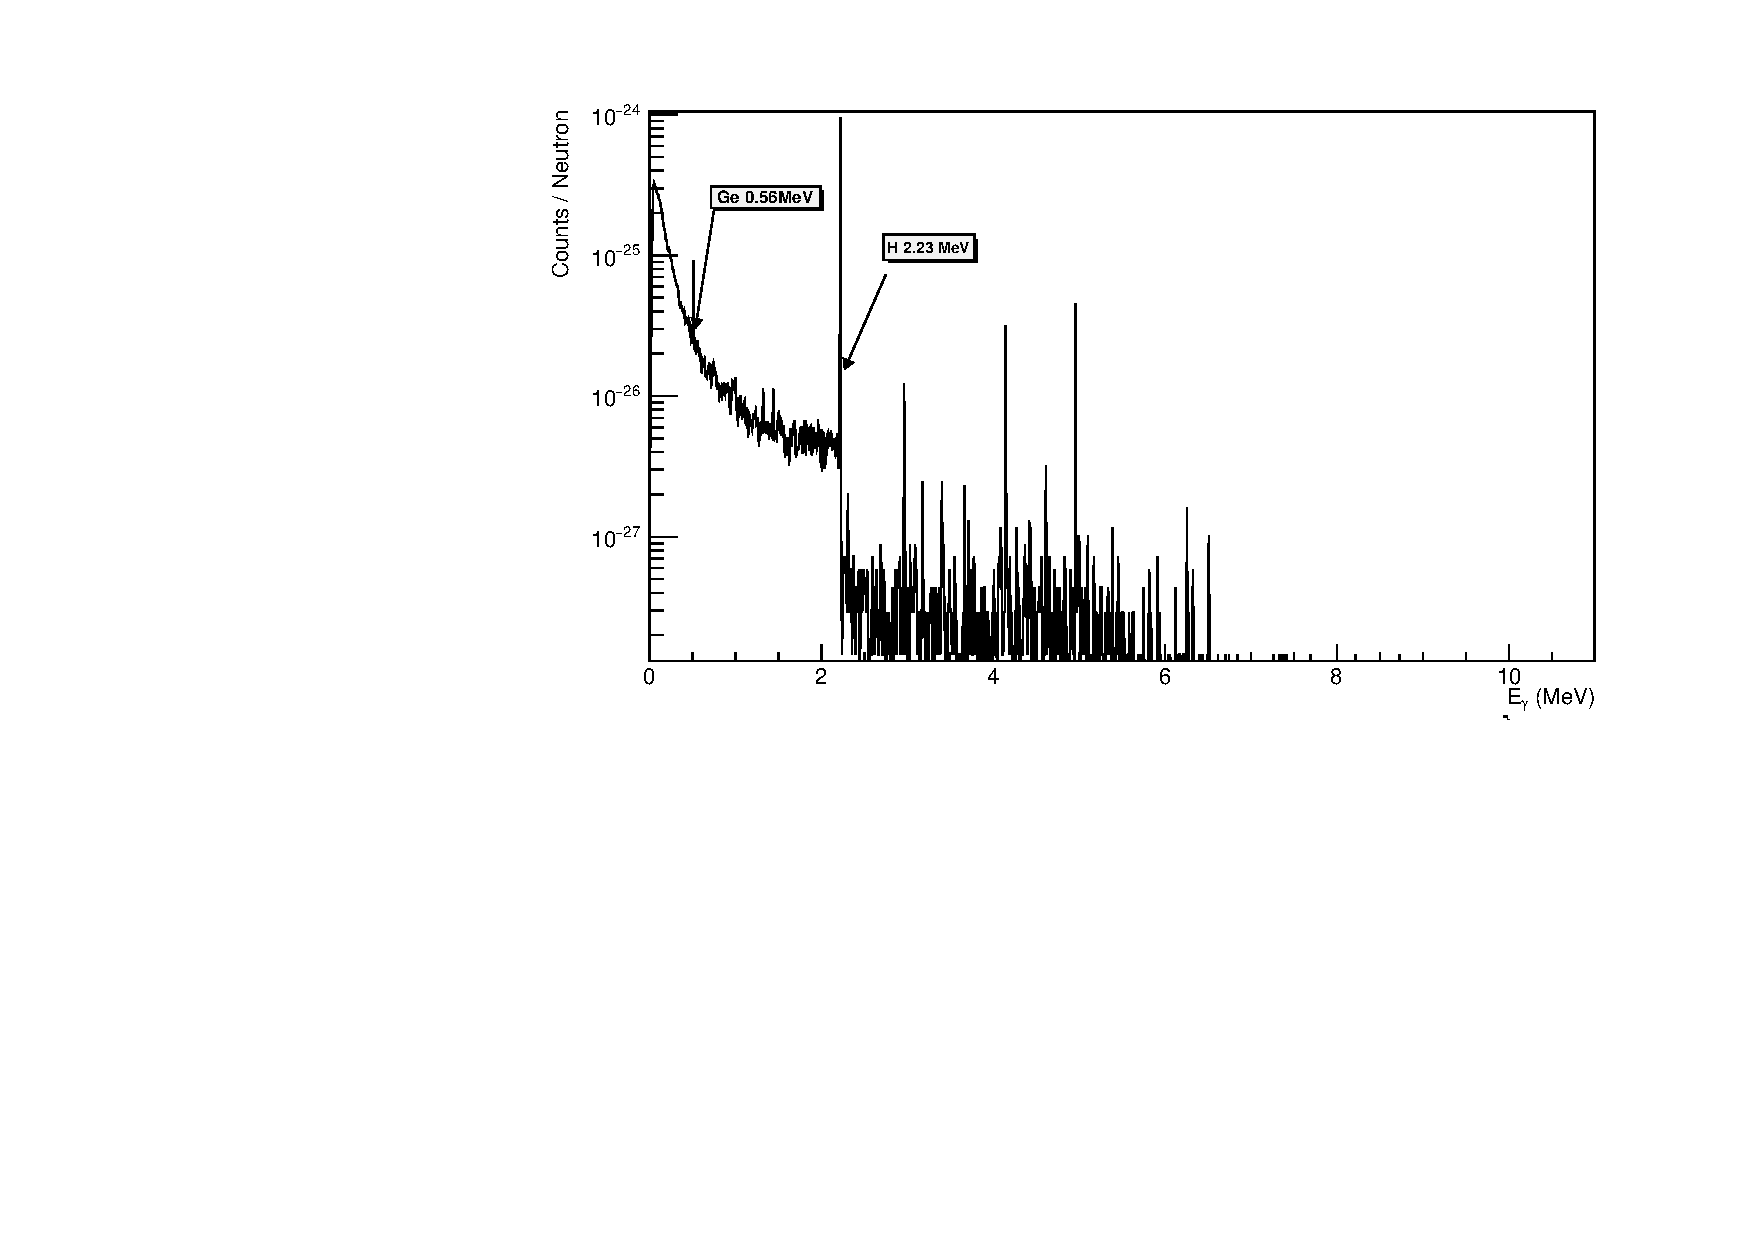
\includegraphics[width=1\textwidth]{res/AuAgS28MeV.pdf}
		\caption{Червона - лінія спектру, набраного за опромінення нейтронами 8.5 МеВ}
		\label{ris:Ag3AuS22_8MeV}	
	\end{figure} 

\subsection{Дослідження $Au(n, \gamma)$ реакцій} 

\subsection{Аналіз спектрів $CuFeS_2$}
	Данний мінерал являеться основною складовою мідної руди, спектор для нього представлений на Рис. ~\ref{ris:CuFeS_2Fon}
	\begin{figure}[hbt!]
		%\vspace{-10pt}
		\centering 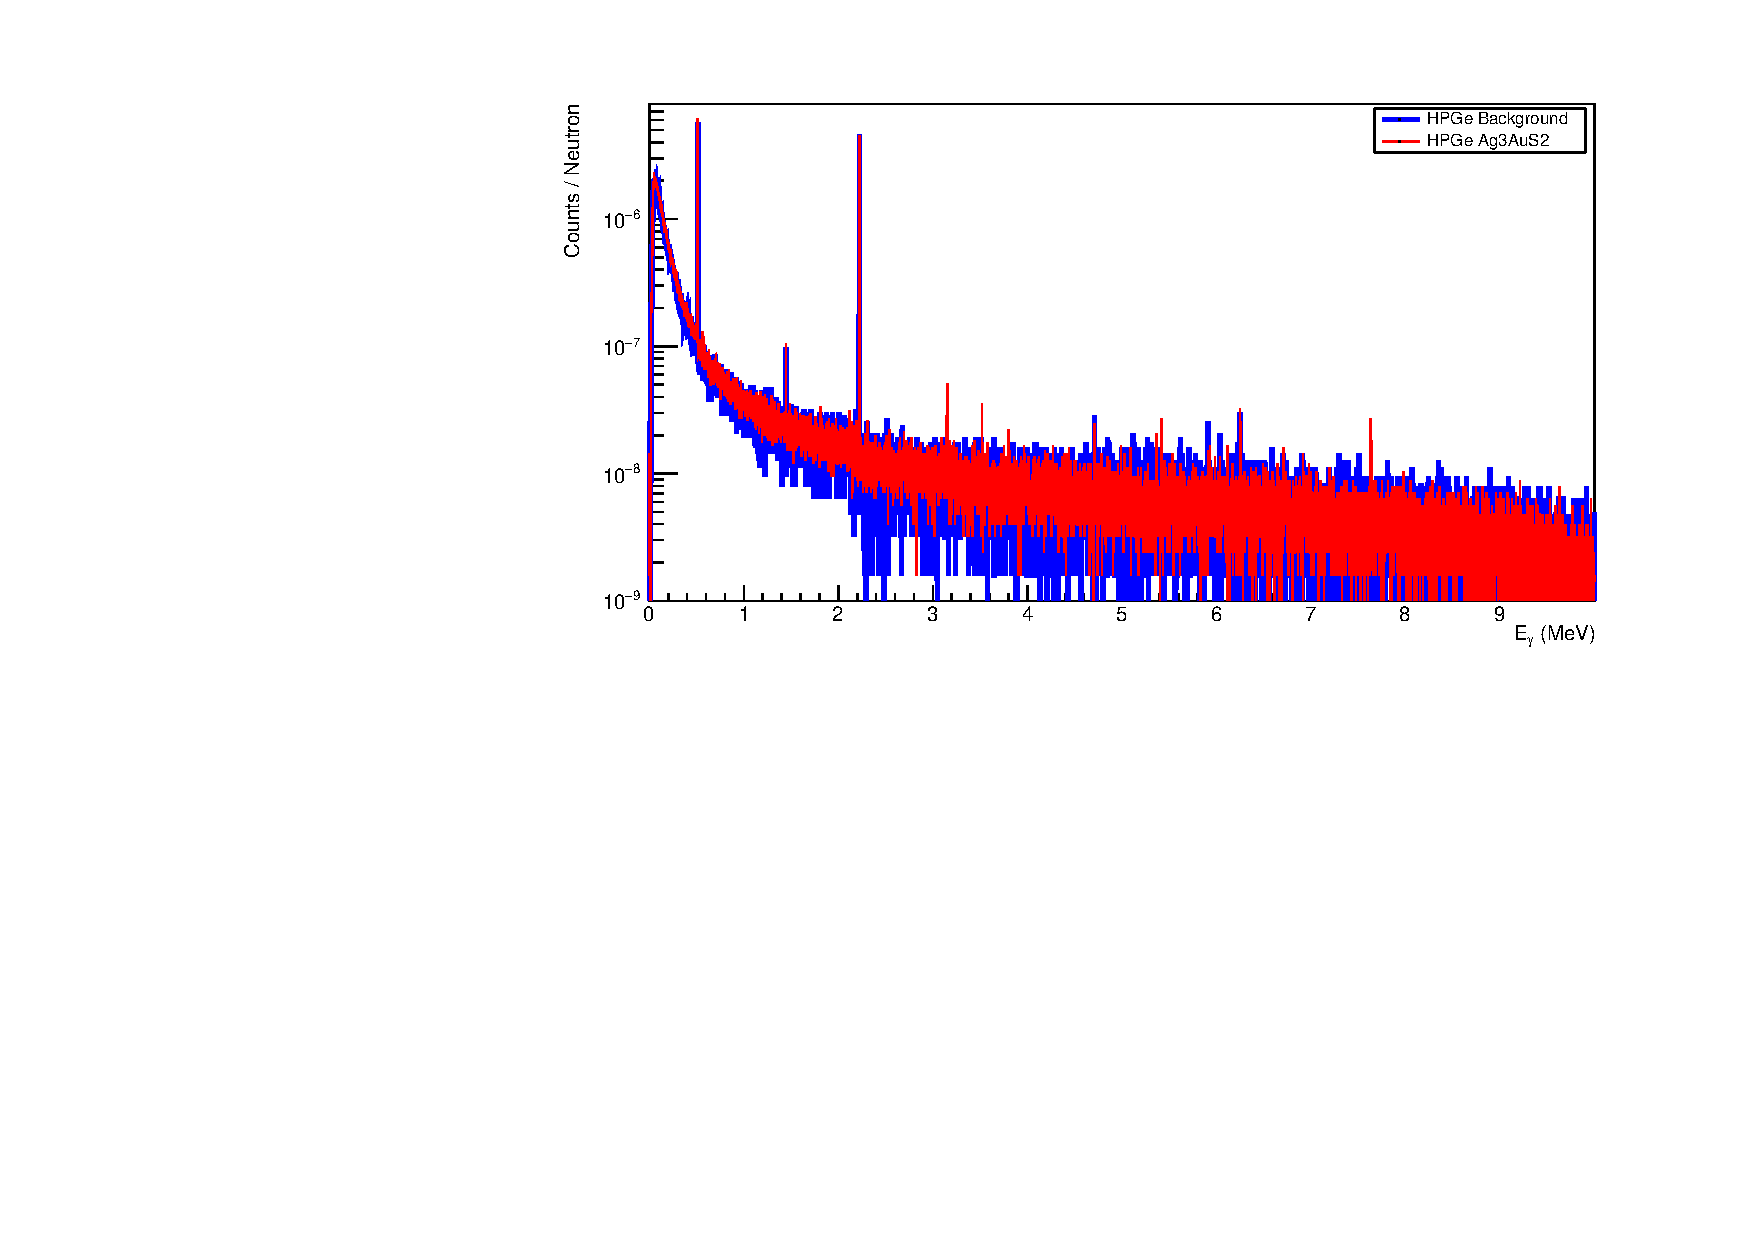
\includegraphics[width=1\textwidth]{res/smCuFeS2FonAll.pdf}
		\caption{Червоним - представлений спектор для $CuFeS_2$. Синім - фону} 
		\label{ris:CuFeS_2Fon}	
	\end{figure} 	
	В високо енергетичній частині спектру можна спостерігати пік для $S_2$
		
\subsection{Аналіз спектру $U^{238}$}
	<Мета набору> Було обрано збіднений уран, з наступним ізотопічним складом $99.27\% -\  ^{238}U$, $ 0.72\% - \  ^{235}U$, $ 0.005\% - \ ^{234}U$, У ході набору було отримано наступний спектор Рисю ~\ref{ris:poorU}
	\begin{figure}[hbt!]
		%\vspace{-10pt}
		\centering 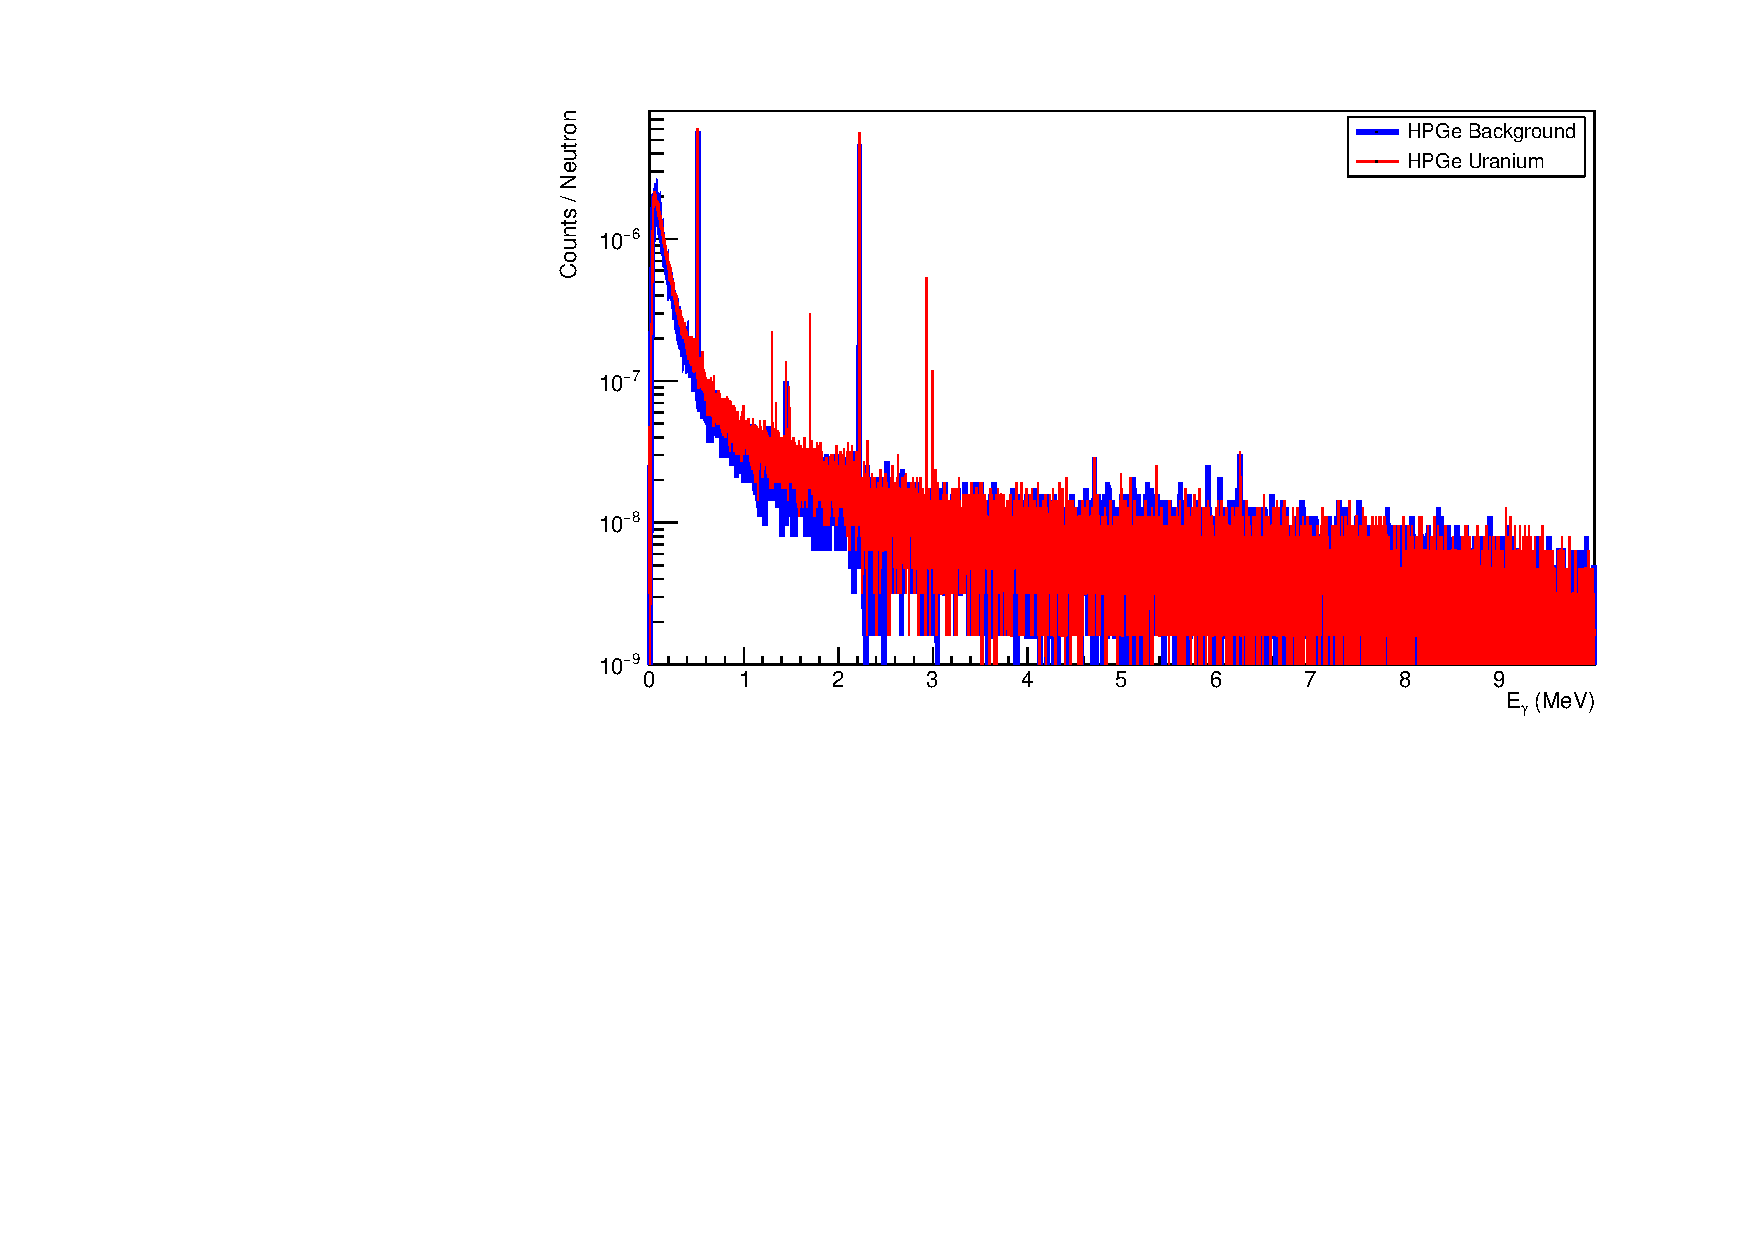
\includegraphics[width=1\textwidth]{res/poorUranium.pdf}
		\caption{Червоним - представлений спектор для $U^{238}$. Синім - фону} 
		\label{ris:poorU}	
	\end{figure} 	 
	На данному спектрі можна спостерігат
	
\newpage 
\section{Висновки}
\setcounter{figure}{0}
У роботі була змодельована спрощена версія системи яка дає змогудосліджувати, та індетифікувати речовини які знаходяться не лише на поверхні океанічного дна, при достатніх потоках нейтронів. Порівнючи з проектом SABAT, де використовувався сетиляційний детектор, була проведена спроба вирішення проблем, які супроводжуються використання напівпровідникових детекторів, та оптимізацією для більш універсального застосування. 
Було встановлено що оптимальна відстань між досліджуваною речовиною та детектором близько 30см. Було проведенно дослідження залежності від енергії нейтронів з джерела, за цими результами було встановлено що джерело можна по-перше розміщувати на більшій відстані, та енергія 14МеВ досить велика для подібного моделювання, тому можна або змешувати енергію але наприклад 2.8 МеВ енергі за низька тому використання ізотопних джерел не можливе. Також враховуючи той факт що я спостерігав взаємодіію нейтронів з чуливим об'ємом детектора є доцільним змінити геометрію, або енергію нейтронів, також приділити додаткову увагу захисту детектора 

\newpage	
%literature
\addcontentsline{toc}{section}{Література}
\begin{thebibliography}{}
	
%	\comment{кометар: це джерело звідки були взяті розміри детектора}  
	\bibitem{1} \textit{R.M. Keyser and T.R. Twomey} - Extended Source Sensitivity and Resolution Comparisons of Several HPGe Detector Types with Low-energy Capabilities \\
	\href{https://www.ortec-online.com/-/media/ametekortec/technical%20papers/high%20purity%20germanium%20detector%20applications%20and%20technology%20developements/extended-source-sensitivity-resolution-comparisons-several-hpge-detector-types-low-energy-capabilities.pdf?la=en}{ HPGe Detector Types}		
	\bibitem{1} \textit{Aatos Heikkinen, Nikita Stepanov Helsinki Institute of Physics, P.O. Box 64, FIN-00014 University of Helsinki, Finland Johannes Peter Wellisch CERN, Geneva, Switzerland} - Bertini intra-nuclear cascade implementation in Geant4
	\href{https://www.slac.stanford.edu/econf/C0303241/proc/papers/MOMT008.PDF}{link}	
	\bibitem{1} \textit{Ю.В. Сереткин, Г.А. Пальянова Институт геологии и минералогии им. В.С. Соболева СО РАН} - ИЗОМОРФНОЕ ЗАМЕЩЕНИЕ СЕРЫ СЕЛЕНОМ И МОРФОТРОПНЫЙ ПЕРЕХОД В РЯДУ $Ag_3Au(Se,S)_2$
	\href{https://www.sibran.ru/upload/iblock/478/478309021b63c0dc426e82c4025e6471.pdf}{link}	
	\bibitem{1} \textit{В. М. Округин1, А. У. Ким} О рудах Асачинского золото-серебряного месторождения
	(Южная Камчатка)
	\href{http://www.kscnet.ru/ivs/publication/volc_day/2014/art51.pdf}{link}	
	\bibitem{1} \textit{Омельчук О.В., Загнітко В.М., Курило М.М.}ПОШУКИ ТА РОЗВІДКА РОДОВИЩ КОРИСНИХ КОПАЛИН КИЇВСЬКИЙ НАЦІОНАЛЬНИЙ УНІВЕРСИТЕТ ІМЕНІ ТАРАСА ШЕВЧЕНКА Навчально-науковий інститут «Інститут геології»
	
\end{thebibliography}

\end{document}
